\documentclass{article}
\usepackage[utf8]{inputenc}
\usepackage{enumitem}
\usepackage{geometry}
\usepackage{graphicx}
\usepackage{float}
\usepackage{listings}

\geometry{a4paper, margin=1in}

\lstset{
    basicstyle=\ttfamily\small,
    breaklines=true,
    frame=single,
    captionpos=b,
    xleftmargin=0.05\textwidth,
    xrightmargin=0.05\textwidth
}

\title{Research Assistant System}
\author{Team G.O.A.T\\
Abdelaziz Ibrahim, Besher Alkurdi, Bishwash Khanal}
\date{}

\begin{document}

\maketitle

\section{Agents' Role and Behaviour}

\subsection{Query Construction Agent}

\textbf{Role:} QueryFormulator | \textbf{Behaviour:} OneShot

\begin{itemize}
  \item Transforms natural language questions into optimized arXiv search syntax
  \item Creates multiple search strategies to increase coverage
  \item Handles both initial queries and refinement requests
  \item Sends queries to the Search Agent
  \item Receives refined queries and suggestions from the Relevant Agent
\end{itemize}

\subsection{Search Agent}

\textbf{Role:} SearchCoordinator | \textbf{Behaviour:} Cyclic

\begin{itemize}
  \item Executes each query against the arXiv API
  \item Parses the results from arXiv API into a structured JSON format
  \item Forwards collected results to the Revelant Agent
\end{itemize}

\subsection{Relevant Agent}

\textbf{Role:} ResultValidator | \textbf{Behaviour:} Cyclic

\begin{itemize}
  \item Evaluates the relevance of each paper against the research question
  \item Checks papers' relevance against a relevance threshold
  \item If the query is to be refined and only a few papers are relevant, send query refinement suggestions to the Query Construction Agent
  \item If sufficient papers are returned, send the papers to the Knowledge Agent
\end{itemize}

\subsection{Knowledge Aggregator Agent}

\textbf{Role:} ContentCollector | \textbf{Behaviour:} OneShot

\begin{itemize}
  \item Receives papers info from the Relevant Agent
  \item Deduplicates the received papers
  \item Saves the results (Papers info) as a JSON file to create a knowledge base
\end{itemize}

\section*{Agent's Communication (Sequence Diagram)}

\begin{figure}[H]
    \centering
    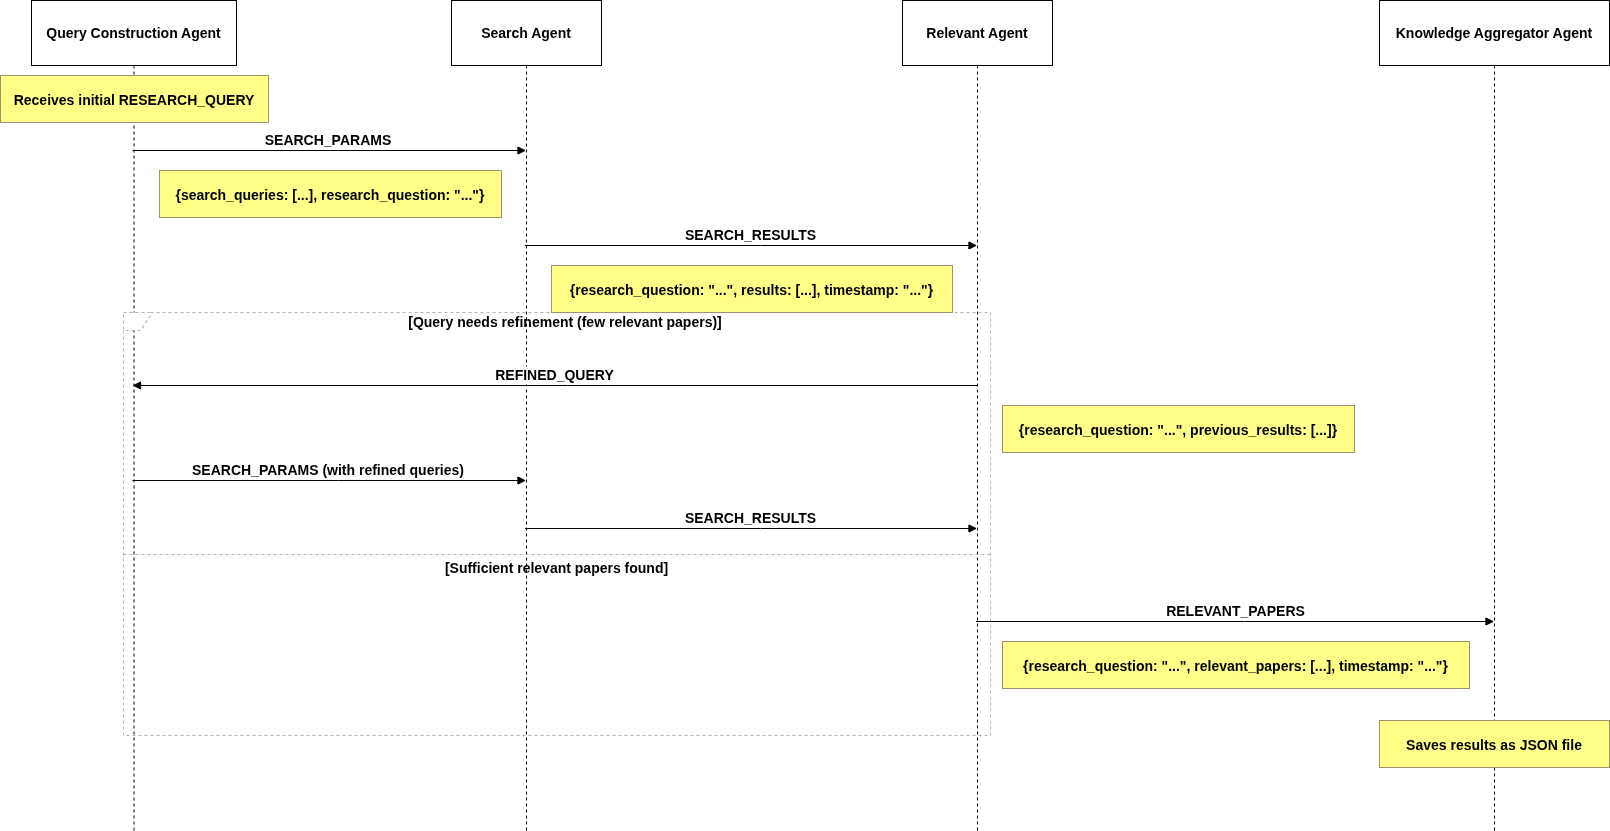
\includegraphics[width=\textwidth]{images/agent_communication.png}
    \caption{Agent Communication Sequence Diagram}
    \label{fig:agent-communication}
\end{figure}

\section*{Screenshots}

\begin{figure}[H]
    \centering
    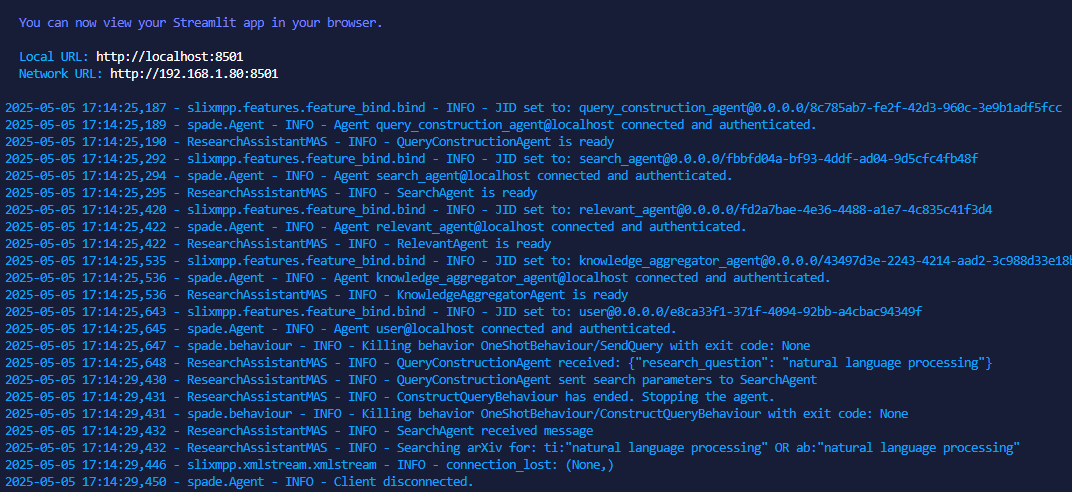
\includegraphics[width=\textwidth]{images/screenshot_1.png}
    \caption{Agent Console Output 1}
    \label{fig:screenshot1}
\end{figure}

\begin{figure}[H]
    \centering
    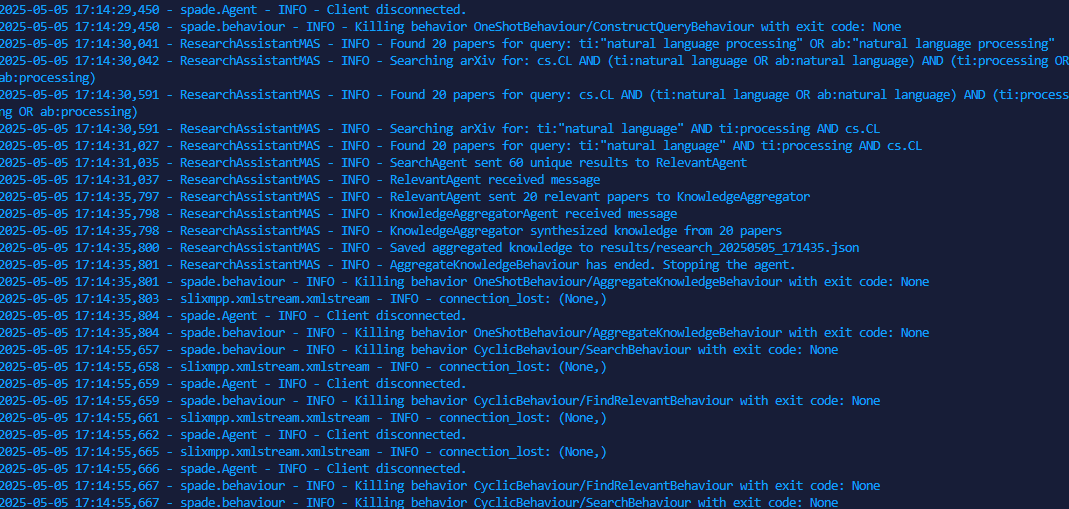
\includegraphics[width=\textwidth]{images/screenshot_2.png}
    \caption{Agent Console Output 2}
    \label{fig:screenshot2}
\end{figure}

\end{document}